% !TEX root = ../../thesis.tex

\chapter{The Uber Basics of \LaTeX{}}%
\label{ch:basics}%
\graphicspath{{chapters/basics/figures/}}

This chapter will briefly expose you to the basics.
It is not a replacement for looking things up online, so make sure you do that too.
I particularly like \url{https://www.overleaf.com/learn} as it is quite digestible.
Make sure you're reading through the actual source files at the same time, as I have left practical comments explaining in more detail than you see here.

I recommend you start by opening \verb|thesis.tex| which is the main file of this template.
Take note of the \verb|\documentclass| command at the top which provides many options for how your document looks.
By default, this template is setup for one-sided A4 paper, 12pt font, a custom font, custom margins, a custom bibliography style, a specific type of heading on each page, and has draft mode turned on (which is why you see line numbers in the margins and a watermark in the footer).
I have included the configurations that I used for my online and print thesis submission variations.

% My personal structure is to have a 'main' file for each chapter, in this case `basics.tex', which then
% includes several other files, one for each section (we will get to structure later on).
% I recommend this method as once your thesis becomes large, having monolithic files can be difficult to manage.

% This is how you directly paste a file into another file.
% ! IMPORTANT NOTE !
% See how this is `input` rather than `include` in thesis.tex? There's an extremely important difference.
% Using `include` will ensure the included content starts on a NEW page. That is, if you're one line over a page and use `include`, it will skip the rest of that page entirely.
% Using `input` will treat it as if you just copy and pasted the file's contents here, not skipping anything.
% !TEX root = ../../thesis.tex

\section{Structure}%
\label{sec:basics-structure}%

\LaTeX{} can organize and number your document automatically with several sectioning commands.
From the highest to the lowest, the commands are:

\begin{itemize}[noitemsep,left=1pt]
  \item \verb|\part{name}|
  \item \verb|\chapter{name}|
  \item \verb|\section{name}|
  \item \verb|\subsection{name}|
  \item \verb|\subsubsection{name}|
  \item \verb|\paragraph{name}|
  \item \verb|\subparagraph{name}|
\end{itemize}

\noindent In your thesis, you are likely to only use \verb|\chapter|, \verb|\section|, \verb|\subsection|, and \verb|\subsubsection|.
The file \verb|basics.tex| defines a chapter, which is represented above by ``Chapter 2''.
This file, \verb|structure.tex|, defines a section, which is represented above as ``2.1''.
When we add subsections, they would be represented as ``2.1.1'' and so on.

The style of these sectioning commands has been customized for this thesis. Look for ``Custom Titles'' in \verb|preamble.tex| for more information.

\subsection*{Unnumbered Sectioning}%
This subsection is not listed in the table of contents and doesn't have a number.
You can achieve this with any of the sectioning commands by appending them with an asterisk.

% !TEX root = ../../thesis.tex

\section{Formatting}%
\label{sec:basics-formatting}%

Formatting text in \LaTeX{} is easy, for the most part.
You can make text \textbf{bold} by wrapping it in \verb|\textbf{}|.
You can make text \textit{italic} by wrapping it in \verb|\textit{}|.
You can \underline{underline} text by wrapping it in \verb|\underline{}|.
These can of course be \textbf{\textit{\underline{combined}}} together.

It is important to be aware that \verb|\textit{}| and \verb|\emph{}| almost always act similar, but in fact do different things in different contexts.
In short, \verb|\emph{}| behaves differently as you nest it in different commands, and some packages may in fact change its behavior.
If you want something that's \textit{definitely} italic, stick with \verb|\textit{}|.

This thesis template also uses the \texttt{soul} package which extends the formatting options you have available.
For example, we can \st{strike through} text by wrapping it in \verb|\st{}|.

It is also worth noting that many special characters in \LaTeX{} have reserved meanings, so you cannot use them verbatim.
Consider, for example, the ampersand (\&), percent (\%), and dollar (\$) symbols.
These characters must be \textit{escaped} by placing a backslash (\textbackslash) before them.
In this case, we would write \verb|\&|, \verb|\%|, and \verb|\$|.

\subsection{Quotes}%
You should \textbf{never} use double quotes directly within \LaTeX{} to wrap quoted text.
Instead, you should insert backticks to the left of the quote, and apostrophes to the right (see \verb|formatting.tex|).
These can both stack indefinitely, so add them to your heart's content!

For example, ``this quote has two backticks before it and two apostrophes after it'' whereas `this quote only has one either side'.
We can also display block quotes as follows:

\begin{displayquote}[][]
  ``This block of text is displayed centered on the page and represents a chonkier block of text than you'd typically quote inline. Here is some more filler text to make this quote much longer. Significantly longer. In fact, so long that I'm not quite sure what to add here other than these padding words.'' 
\end{displayquote}

\subsection{Lists}%
Use the \verb|enumerate| environment to list things by number.

\begin{enumerate}[noitemsep,topsep=0pt]
  \item Items within enumerate blocks are numbered automatically.
  \item By default, this starts at 1, but it can be configured with the \texttt{enumitem} package.
  \item There's no limit to the length of these, as long as they are one line.
\end{enumerate}

\vspace{5pt}

\noindent Use the \verb|itemize| environment to list arbitrary things by bullet point.

\begin{itemize}[noitemsep,topsep=0pt]
  \item This is an example bullet point.
  \item So is this one.
  \item And this one!
\end{itemize}

\vspace{5pt}

\noindent You can use the \verb|description| environment to list items with descriptions, although I usually tend to do this by hand.

\begin{description}[noitemsep,topsep=0pt]
  \item[The Title] A short description that follows.
  \item[Another Title] This can be any length, as long as it's one line.
\end{description}

\vspace{5pt}

\noindent These environments can be nested and configured quite deeply, so do look them up!

\subsection{Footnotes}%
You can add footnotes to any text by using the \verb|\footnote{}| command.
Do \textbf{not} add a space before the command as a superscript number will be inserted in its place.

By default, this thesis template will place all footnotes at the \textbf{end} of the document, delineated by which chapter they appear in.
This is a personal preference and some people prefer to see them on the same page at the bottom.
I dislike having them on the same page as they can begin to take up some serious space and introduce formatting oddities, whereas when they are at the end of the document, their length and quantity really doesn't matter.
Look at \verb|preamble.tex| for more information on how to toggle between these two modes.

Here are several examples of footnotes.
Popular search engines include Google\footnote{Available at \url{https://www.google.com}.}, Bing\footnote{Available at \url{https://www.bing.com}.}, and DuckDuckGo\footnote{Available at \url{https://duckduckgo.com}.}.
Also note that this template includes a custom \verb|\AsOfToday| command that you can use to automatically specify `today' when building your document.
It is helpful for specifying when a link was last valid, for example\footnote{Imagine I'm talking about an amazing website available at \url{www.website.com} \AsOfToday.}.

% !TEX root = ../../thesis.tex

\section{Figures \& Tables}%
\label{sec:basics-figures_and_tables}%

\subsection*{Figures}%
Figures are typically made up of a \verb|figure| environment, a \verb|\centering| command to keep the content aligned in the middle of the page, an \verb|\includegraphics| command to insert the image itself, a \verb|\caption| command to insert a caption, and a \verb|\label| command to give it a referenceable name, which we will look at later.

Figure~\ref{fig:basics-skyrim_book} shows how to insert a single figure with a caption.
The image is inserted using the \verb|\includegraphics| command, where its \verb|width| option is used to size the image relative to the text's maximum width.
A caption is also added and placed below the image with the \verb|\caption| command, and \verb|\label| is used to provide an anchor that we can reference in text, as the start of this paragraph did.
The position of the image is controlled by both its literal position in the \LaTeX{} source as well as an optional argument to the \verb|\figure| environment.
Placement of figures in \LaTeX{} can be tricky and they can often end up where you don't want them to!

% Note how this is wrapped in the 'figure' environment. The "!htbp" is a positioning hint. Have a search online for more details.
\begin{figure}[!htbp]
  % This ensures that the image is centered on the page. You almost always want this.
  \centering
  % This is now we include graphics. The argument in the square brackets defines the image width as a 0-1 percentage of the text's width.
  % You can also use direct sizes here, too, but this is most common. The actual image is specified WITHOUT its extension.
  % Remember in the parent basics.tex file, we set graphics path as "\graphicspath{{chapters/basics/figures/}}"?
  % The images are relative to that. As other chapters refined graphicspath, they become relative to that path, and so on.
  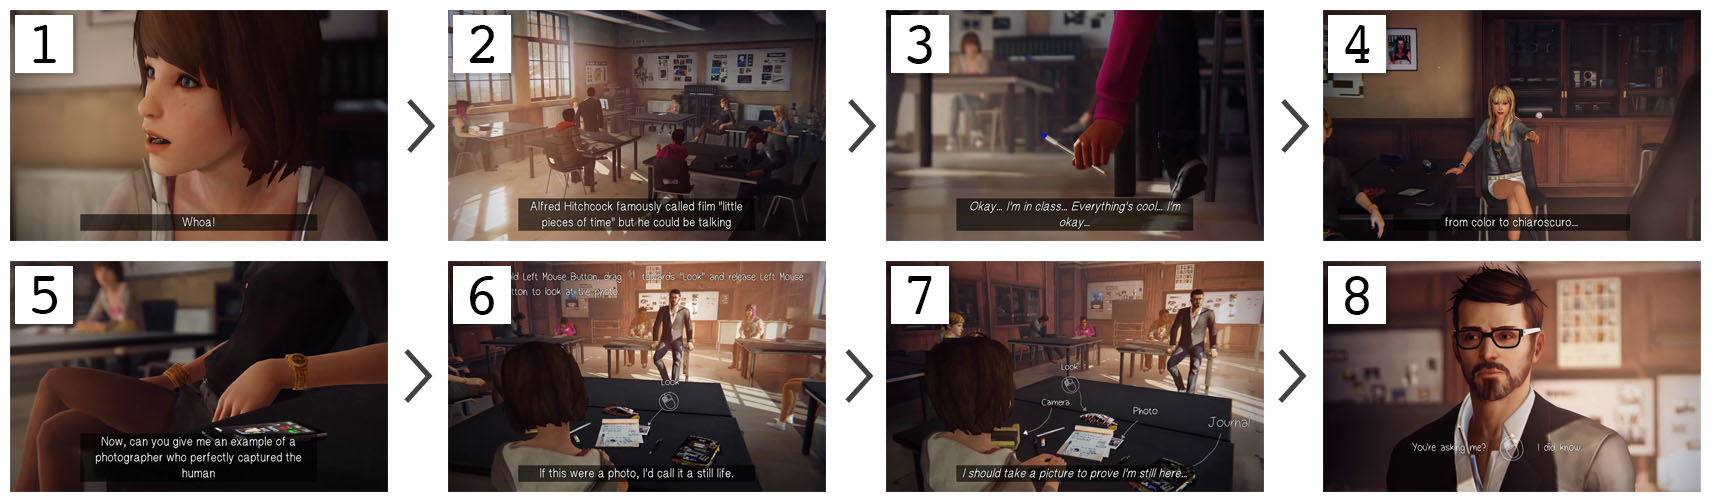
\includegraphics[width=1.0\textwidth]{lis-overview}
  % This caption appears below the image. If you want it above, simply move the line up above \includegraphics.
  \caption{A high-level overview of the \textit{Life is Strange} sequence. 1.\ Max wakes up in class. 2.\ A lecture is taking place. 3.\ Stella drops her pen. 4.\ Taylor bullies Kate. 5.\ Victoria's phone vibrates. 6.\ Max's desk interactions. 7.\ Max's camera usage prompt. 8.\ Max's questioning for disturbing class.}%
  % This defines a label that we can \ref{} later, which we will be doing!
  \label{fig:basics-skyrim_book}
\end{figure}

Figure~\ref{fig:basics-obra} shows how to stack multiple images together in one figure either horizontally or vertically.
We can even reference its parts like Figure~\ref{fig:basics-obra_1} and Figure~\ref{fig:basics-obra_2}.
In this template, this is achieved with the \verb|subfig| package and its \verb|\subfloat| command.

% Notice how there are TWO labels here. This lets us reference Figure X.A, X.B separately.
\begin{figure}[!htbp]
  \centering
  
  % Notice how we're using the \subfloat command to insert a caption, then \includegraphics and \label are used inside its brackets.
  \subfloat[Entering Part 4 of Chapter IV by interacting with Bun-Lan Lin's body. Parts 1, 2, and 3 unavailable at this point.]{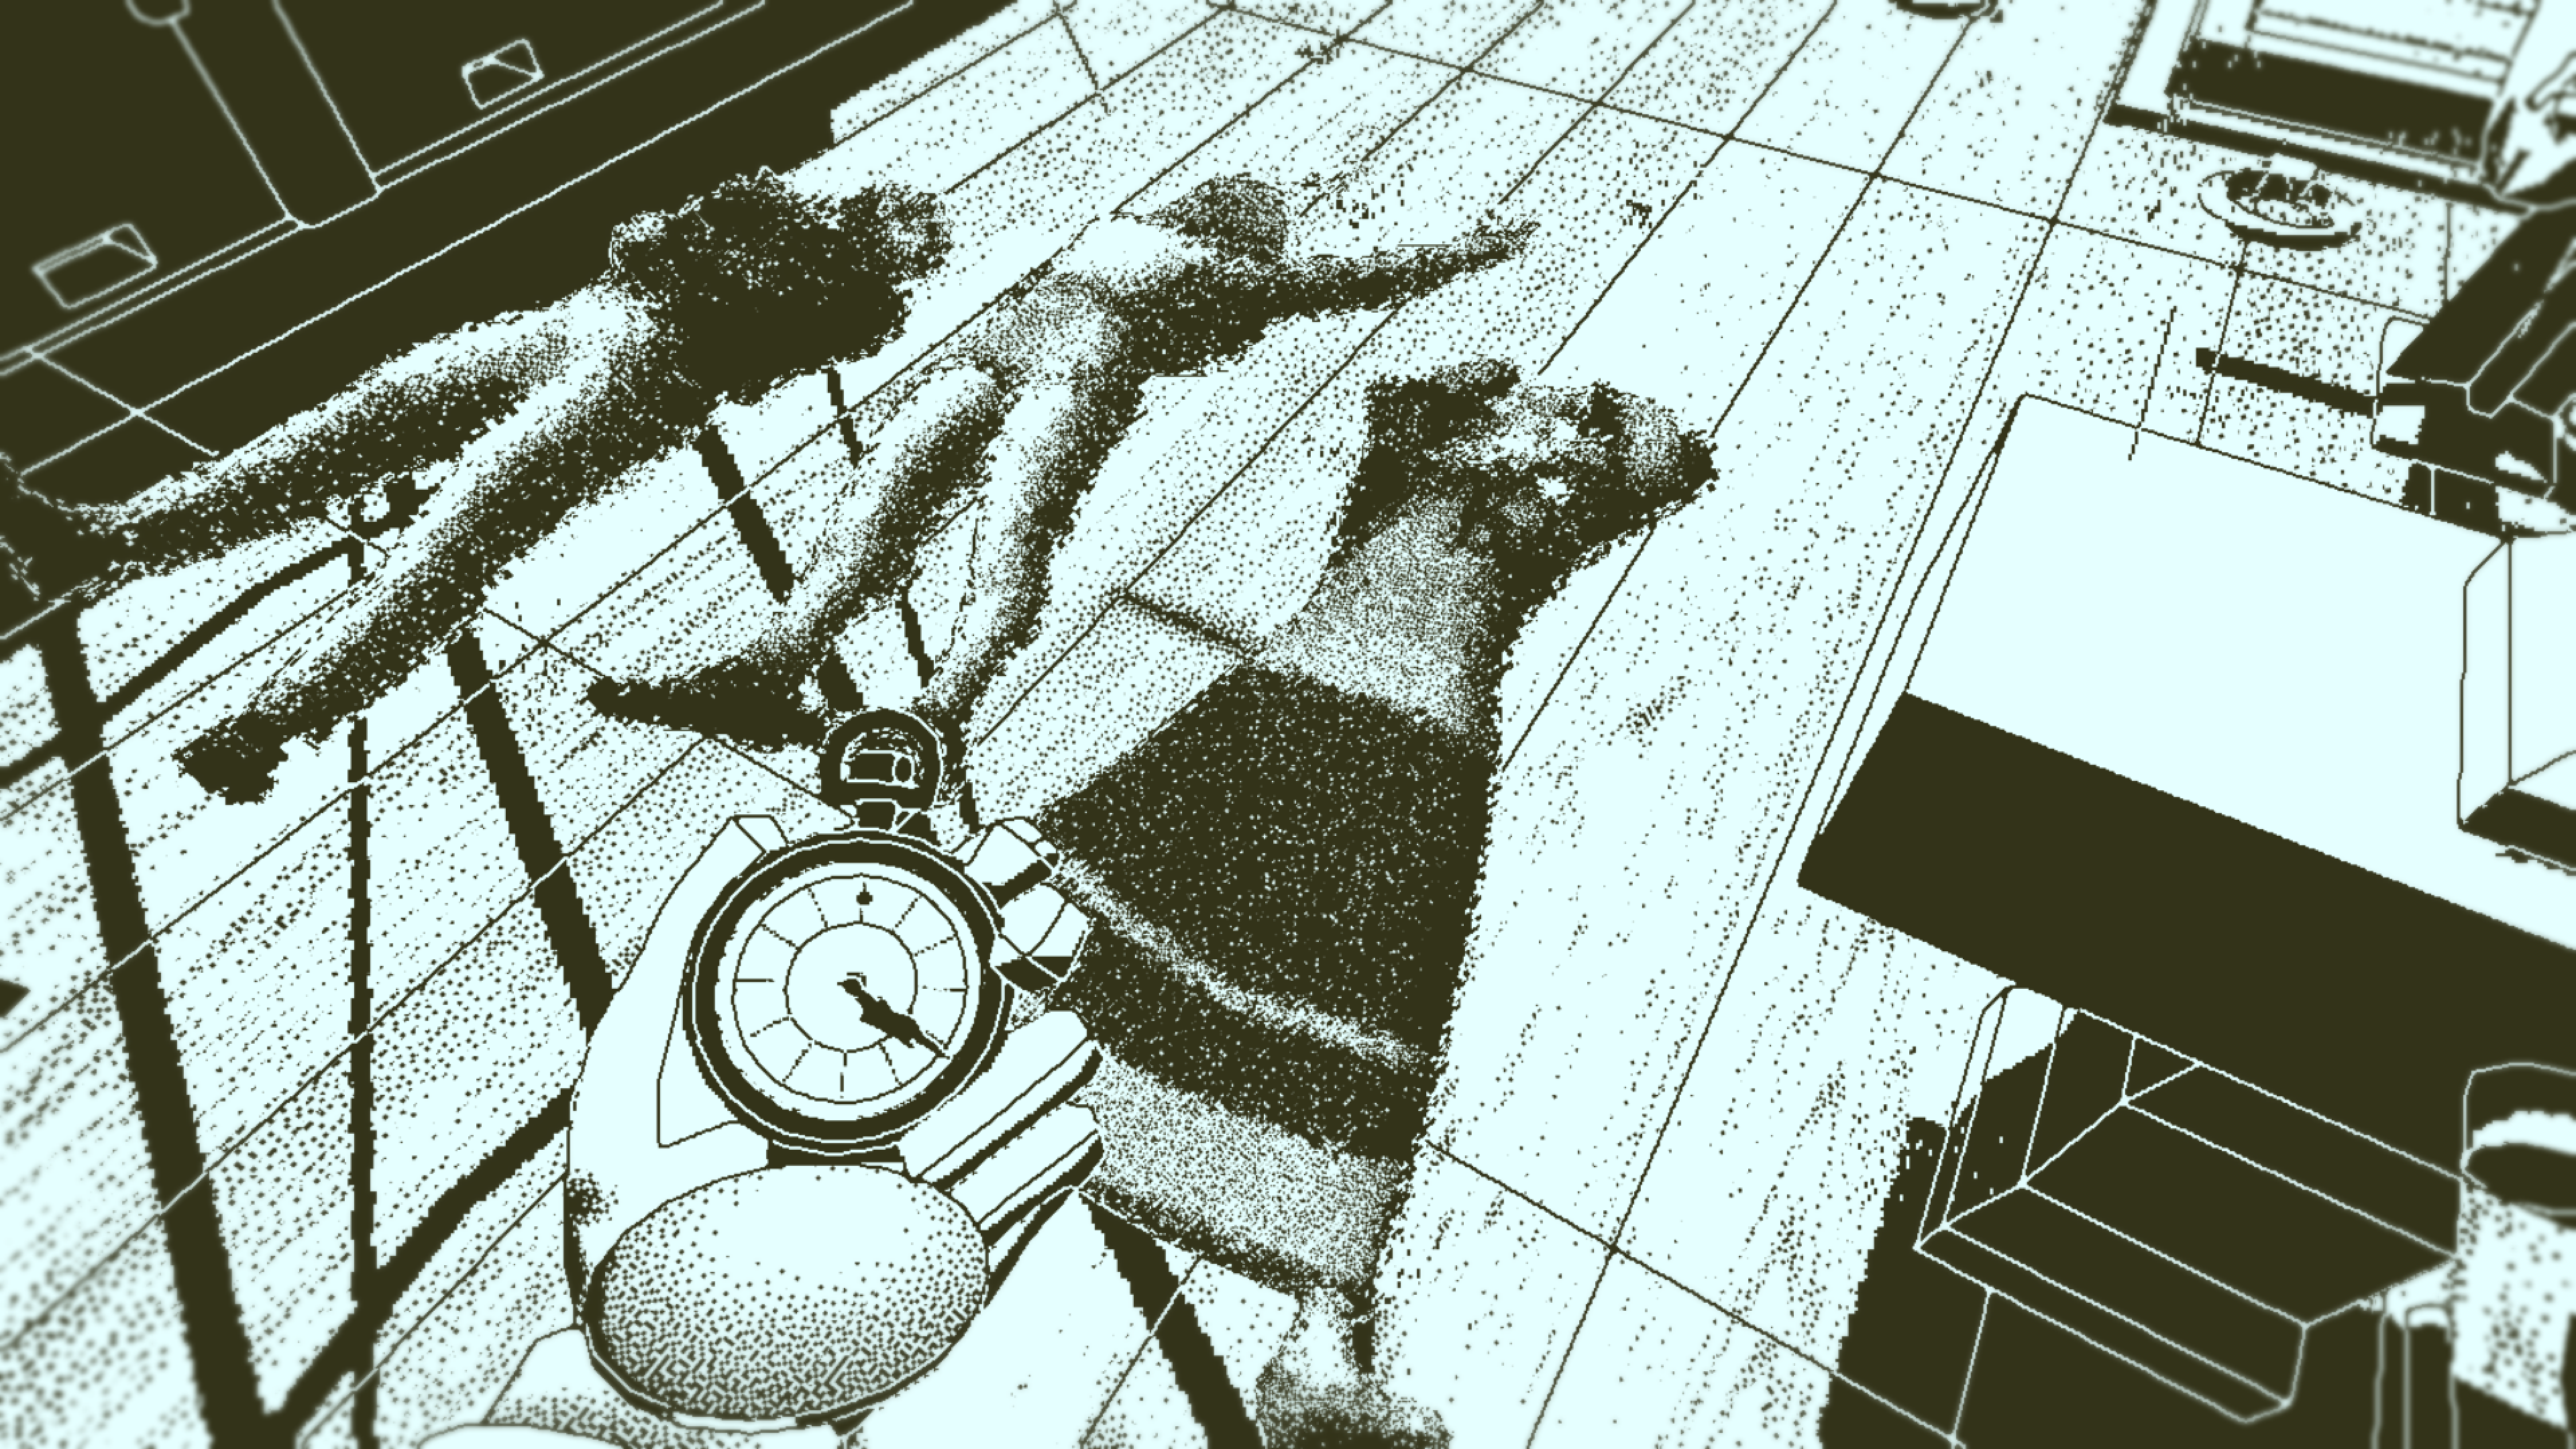
\includegraphics[width=.48\textwidth]{obra-1}\label{fig:basics-obra_1}}
  % This helps with spacing between horizontal images.
  \quad
  % Notice how the size is less than 50% (0.48 in this case). This is so that there's room around each image for spacing.
  % If you just used 50%, they would stack vertically instead of horizontally.
  \subfloat[Entering Part 2 from within Part 4 by locating and interacting with Patrick O'Hagan's body.]{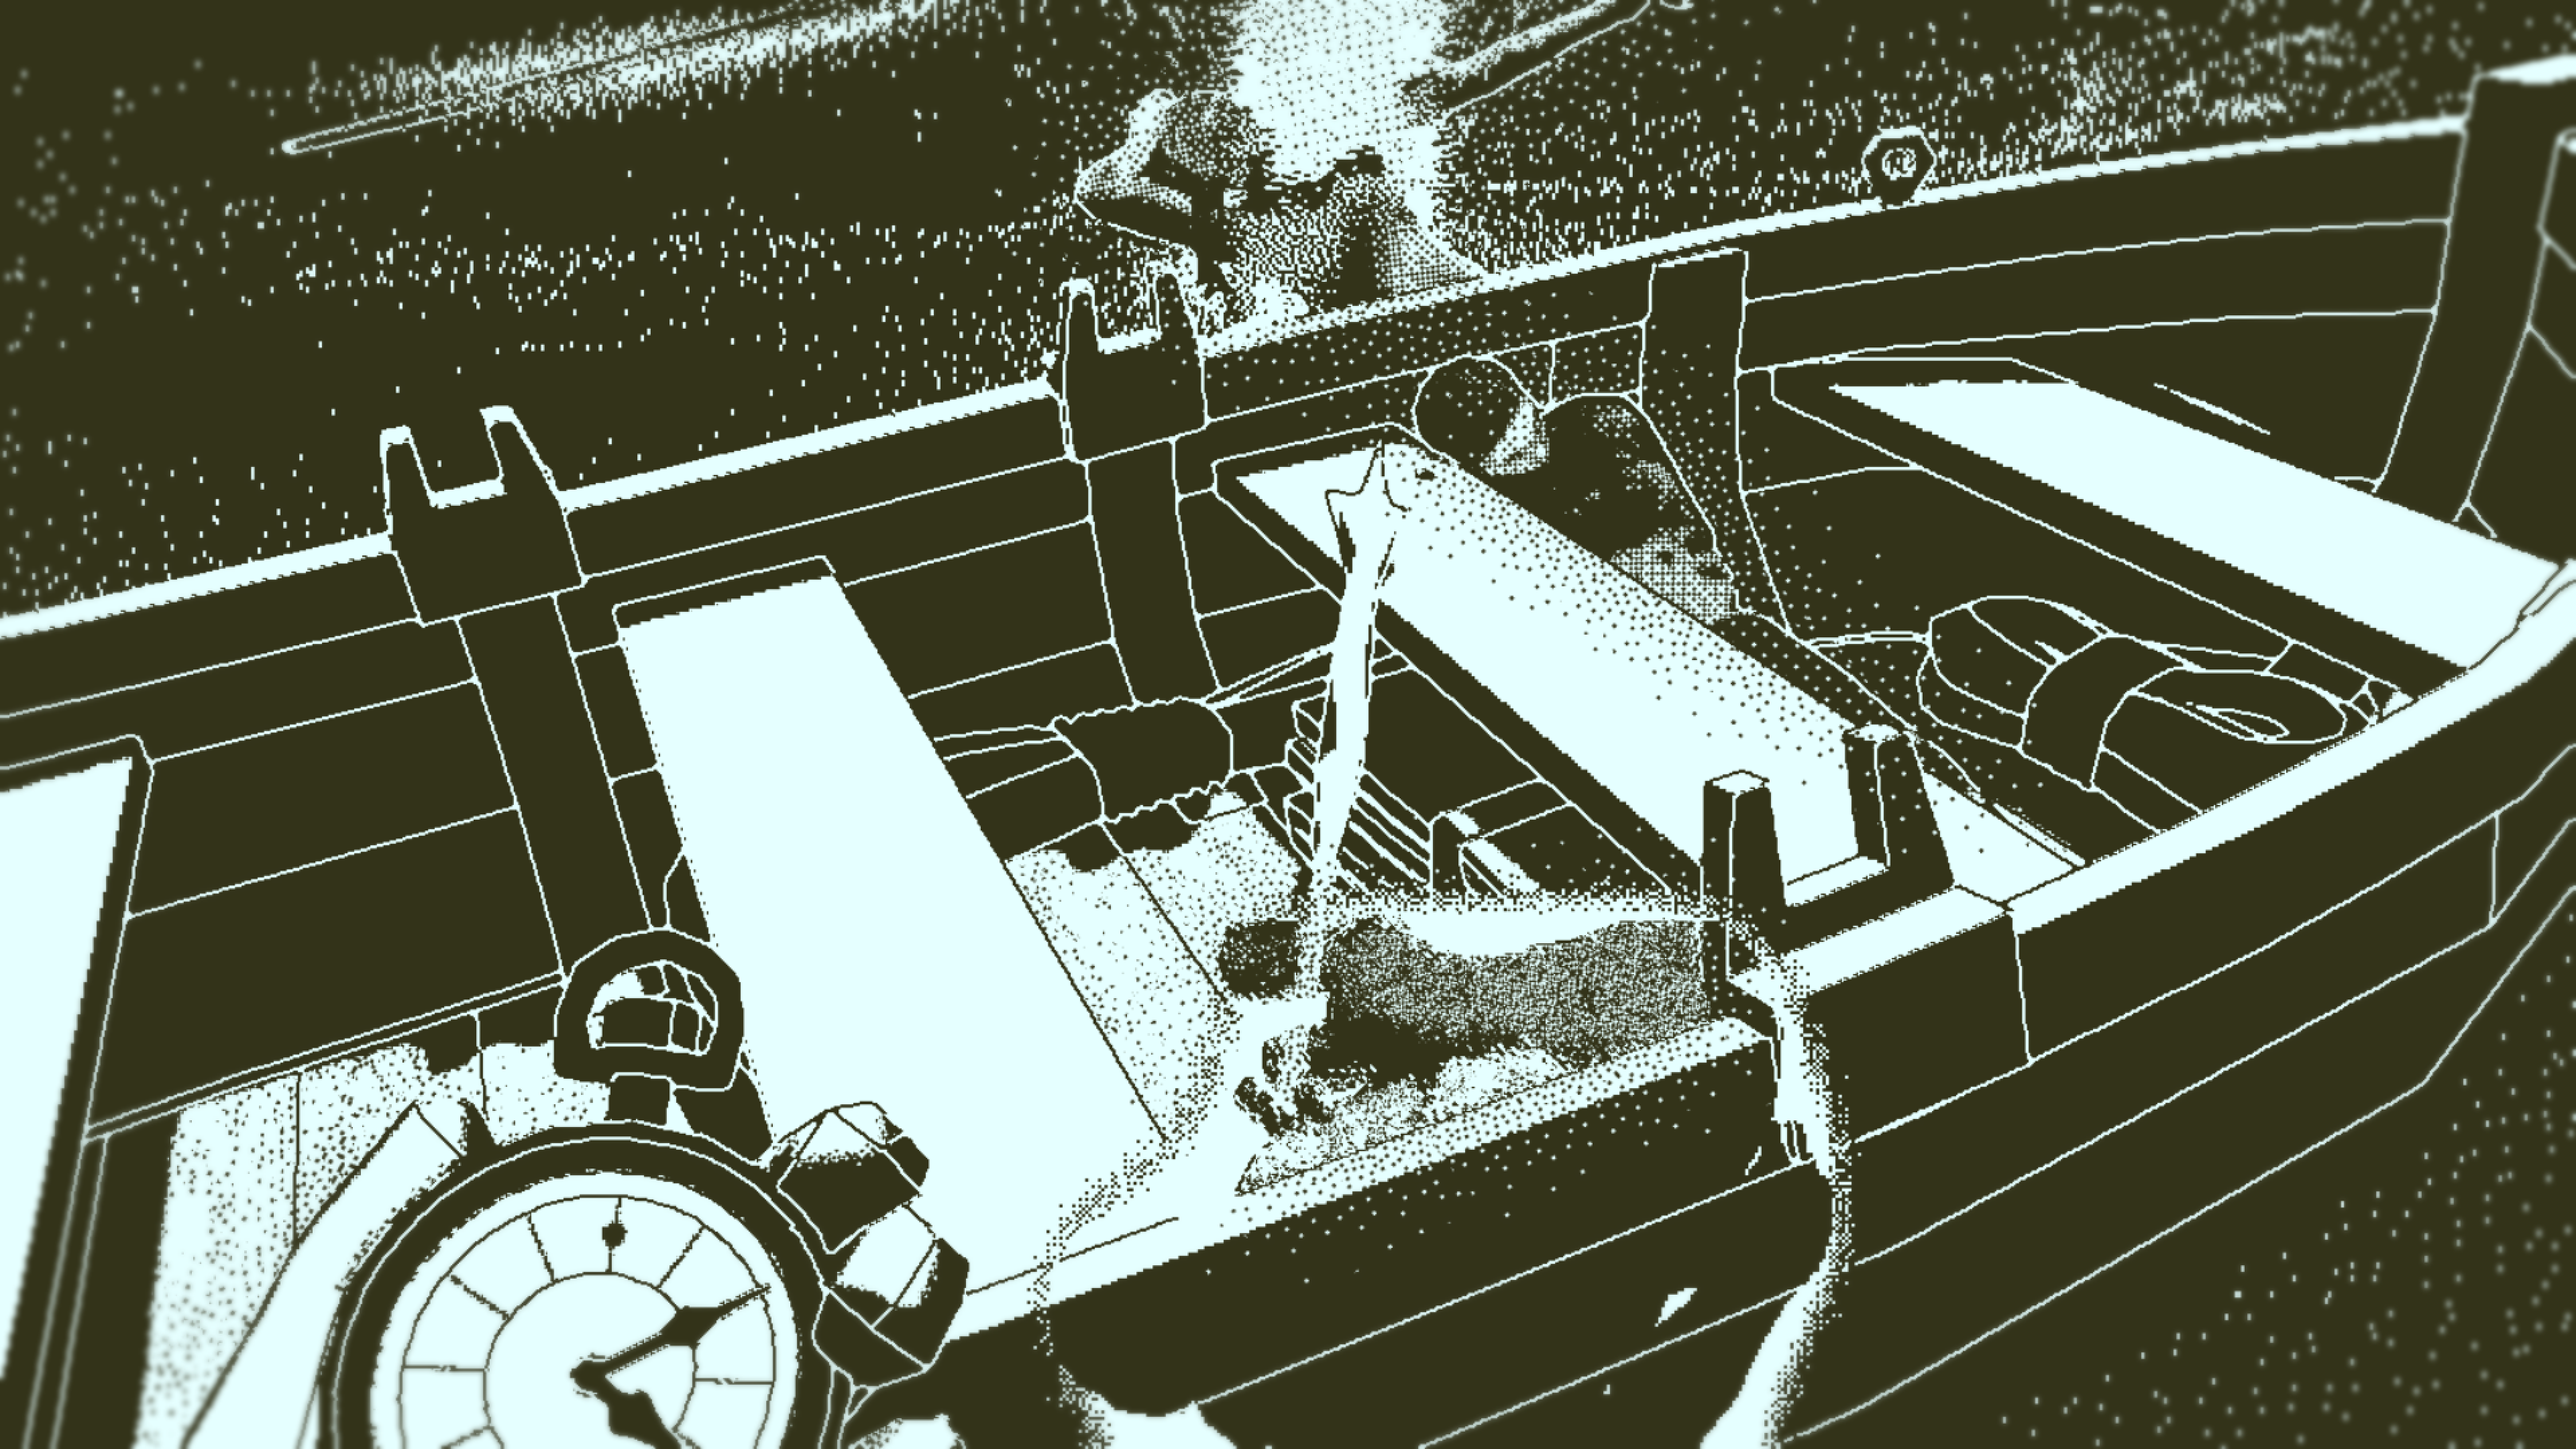
\includegraphics[width=.48\textwidth]{obra-2}\label{fig:basics-obra_2}}
  \caption{A player in \textit{Return of the Obra Dinn} entering into Part 4 of Chapter IV by interacting with Bun-Lan Lin's body on the main deck. From Part 4, they discover Patrick O'Hagan's body, which can take them to Part 2 of the same Chapter.}

  \label{fig:basics-obra}
\end{figure}

\subsection*{Tables}%
Tables can be a nightmare in \LaTeX{}, but once working, can give very elegant results.
I strongly recommend you look up how to create effective tables online.
This thesis template already comes with several packages that enhance or otherwise improve tables.

You should always wrap your tables in the \verb|table| environment if you want them to have captions and be referenceable.

Table~\ref{table:basics-table_1} shows a relatively complex table.
Check out the \LaTeX{} source for more details which explains how everything works.
Tables often look best at the \textbf{top} of a page, but here they are forced to be nearby.

% This is just like {figure} but with a table inside. Captions and labels are *typically* at the top of a table.
\begin{table}[!htbp]
  \centering
  \caption{A relatively complex table with multi-column headings, skipped headings, automatic width columns, and more.}%
  \label{table:basics-table_1}
  
  % If you want your tables to be smaller (or larger), you can insert this (or another size) INSIDE the table environment.
  % \footnotesize

  % The first parameter specifies the overall width of the table.
  % The second complex looking parameters determine the columns and their sizes/behaviors.
  \begin{tabularx}{\linewidth}{>{\raggedright\arraybackslash}p{0.63\linewidth} *3{X} | *3{X}}
    % This is the top row. Notice how there's an empty &. This skips the first column.
    % The multicolumn{3} commands merge 3 cells into one piece of text.
    & \multicolumn{3}{c}{Topic A} & \multicolumn{3}{c}{Topic B}\\
    % This is the second line of the heading which doesn't skip any columns.
    Summarizing Title & A & B & C & A & B & C\\
    % This adds a full width line to segment the header from the rest of the table.
    \toprule
    
    % Here are the table entries. Notice how all but the last one end in \\. This is how you start a new row.
    Mauris porttitor, arcu id sagittis & 10 & 0 & 12 & 6 & 0 & 7\\
    Nullam erat mauris, consectetur nec & 0 & 8 & 0 & 0 & 5 & 0\\
    Integer elementum lobortis ligula vitae & 7 & 2 & 0 & 7 & 2 & 0\\
    Maecenas id magna in neque & 1 & 1 & 5 & 1 & 1 & 5\\
    Curabitur tincidunt est vel magna & 0 & 5 & 2 & 0 & 5 & 2
    \end{tabularx}
\end{table}

Table~\ref{table:basics-discoverable_narrative_table} show below has a much more complex setup with custom colors and nested multiline cells.
In this table, there are no headings at the top, but instead the left column has been used.
Each cell to the right of the headings column has a title and a subtitle within it.
Typically, adding line breaks into a cell is challenging and can introduce formatting troubles.
This table uses the \verb|makecell| package to create custom cells with line breaks in them which \LaTeX{} treats as a single cell.

\definecolor{DNHeaderColor}{HTML}{568eae}
\definecolor{DNRowColor1}{HTML}{ffffff}
\definecolor{DNRowColor2}{HTML}{f5f6f8}
\newcommand{\DNCell}[1]{\Gape[2pt][2pt]{#1}} % Arguments to Gape are vertical spacing around the cell up then down.
\newcommand{\DNHeaderCol}{\color{white}\cellcolor{DNHeaderColor}}
\newcommand{\DNRowColOne}{\cellcolor{DNRowColor1}}
\newcommand{\DNRowColTwo}{\cellcolor{DNRowColor2}}
\begin{table}[!htbp]
  \centering
  \caption{\textit{Discoverable Narrative's} four-dimensional descriptor consisting of \textit{Tangibility}, \textit{Functionality}, \textit{Clarity}, and \textit{Delivery}.}%
  \label{table:basics-discoverable_narrative_table}

  \sffamily % Only for this scope.
  \begin{tabularx}{\linewidth}{r l X}
    \DNHeaderCol\textbf{Tangibility} &
    \DNRowColOne\DNCell{\makecell[l]{Tangible\\{\footnotesize Attached to an in-game object.}}} &
    \DNRowColOne\makecell[l]{Intangible\\{\footnotesize \textbf{Not} attached to an in-game object.}}\\

    \DNHeaderCol\textbf{Functionality} &
    \DNRowColTwo\DNCell{\makecell[l]{Narrative\\{\footnotesize Primary purpose is for narrative.}}} &
    \DNRowColTwo\makecell[l]{Mechanical\\{\footnotesize Primary purpose is \textbf{not} for narrative.}}\\

    \DNHeaderCol\textbf{Clarity} &
    \DNRowColOne\DNCell{\makecell[l]{Explicit\\{\footnotesize Clearly and well defined.}}} &
    \DNRowColOne\makecell[l]{Implicit\\{\footnotesize Abstract and interpretative.}}\\

    \DNHeaderCol\textbf{Delivery} &
    \DNRowColTwo\DNCell{\makecell[l]{Active\\{\footnotesize Requires interaction.}}} &
    \DNRowColTwo\makecell[l]{Passive\\{\footnotesize Is observed or experienced.}}\\
  \end{tabularx}
\end{table}

For more advanced tables that spread across multiple pages, you should check out the included \verb|xltabular| package.

% !TEX root = ../../thesis.tex

\section{Citing \& Referencing}%
\label{sec:basics-citing_and_referencing}%

\subsection*{Citing External Works}%
When citing external works, you must firstly add an entry to a \verb|.bib| file.
This template includes \verb|mypubs.bib| for your own works and \verb|\references.bib| for other works.
Once you have added an entry to a \verb|.bib| file, you are ready to cite it in text.

By default, this template uses a custom bibliography style named \verb|ieeecustom| which derives from the original \verb|ieee| style.
The only modification is that it uses \textit{Sentence Case Like This} rather than \textit{Regular case like this}.
Feel free to change this in \verb|preamble.tex|.

\begin{table}[!htbp]
  \centering
  \caption{A list of the most common citation commands.}%
  \label{table:basics-citing_examples}
  
  \begin{tabular}{>{\raggedright\arraybackslash}p{0.55\linewidth} >{\raggedright\arraybackslash}p{0.35\linewidth}}
    \textbf{Command} & \textbf{Example}\\
    \toprule

    \verb+Example~\cite{green_useoftools_2021}+ & Example~\cite{green_useoftools_2021}\\
    \verb+\citeauthor*{green_useoftools_2021}+ & \citeauthor*{green_useoftools_2021}\\
    \verb+\citeauthor{green_useoftools_2021}+ & \citeauthor{green_useoftools_2021}\\
    \verb+\citeyear{green_useoftools_2021}+ & \citeyear{green_useoftools_2021}

    \end{tabular}
\end{table}

Table~\ref{table:basics-citing_examples} shows several of the most common citation commands and an example of each.
Take careful note of the \verb|~| symbol before \verb|\cite|.
This character is a \textit{non-breaking space} which means that the word before it, in the above case ``Example'', will not be separated from the text that follows, in the above case the \verb|\cite| command.
Practically, this means that you will never have a word and its citation separate from one another at a line break, for instance.
It is important to note that \verb|~| \textbf{replaces} a regular space between the two, but visually appears identical; only its behavior changes.

It is also possible insert a complete citation by using the \verb|\fullcite| command:

\medskip

\noindent\fullcite{green_useoftools_2021}


\subsection*{Citing Internal Elements}%
If you instead want to reference something \textbf{internal} to the document, such as a figure, table, or chapter and so on, then you will be using the \verb|\ref| command.

If you look back at the tables, figures, and section headings in the \LaTeX{} code so far, you'll see liberal use of the \verb|\label| command.
This is what creates an anchor that we can use \verb|\ref| to refer to.

I may want to raise something discussed in Chapter~\ref{ch:introduction}, or a specific section such as \S\ref{sec:basics-formatting}.
Tables and figures are exactly the same --- consider Table~\ref{table:basics-citing_examples} or Figure~\ref{fig:basics-skyrim_book}.

Again note the use of \verb|~| as a non-breaking space before \verb|\ref|.
The exception to this is when using the \verb|\S| command (\S), as that symbol typically does not have a space at all.

% !TEX root = ../../thesis.tex

\section{Other Tips}%
\label{sec:basics-other}%

\subsection{Dummy Text / Lipsum}%
If you're blocking out structure and want some filler text, you can use the \verb|\lipsum| command.
Make sure to look up the package documentation on ctan\footnote{\url{https://www.ctan.org/pkg/lipsum}} as it's very flexible.

\lipsum[4]


\subsection{Code Snippets}%
This template uses the \verb|listings| package for inserting code snippets both inline and as blocks/figures.
Again, check the documentation on ctan, which I recommend any time you have questions about a package.

\begin{lstlisting}[language=c++, numbers=left, caption={Checking if a number is even using bit magic.}]
bool isEven( const unsigned int uValue ) {
  return (uValue & (uValue - 1)) == 0;
}
\end{lstlisting}

An alternative package to try is \verb|minted| which you may prefer over \verb|listings|.
It is not included in this template, so you will have to include it manually.


\subsection{Local Environment}%
I do not recommend using Overleaf for your thesis, but instead recommend setting up a local development environment.
This is because you are likely to hit the compilation time limit on Overleaf at some point late in your thesis, and switching environments last second could be a significant disturbance.
Moreover, in my own thesis I've used several advanced features or packages that outright crash Overleaf.
On the flip side, I do recommend having a blank version of this template on Overleaf so that you can quickly play around with formatting (such as building a complex table) and get instant feedback on errors and visuals.

To get \LaTeX{} on your machine, you can visit the main \LaTeX{} download page at \url{https://www.latex-project.org/get} and choose your operating system appropriately.
Personally, I use MiKTeX\footnote{\url{https://miktex.org}} on Windows and MacTeX\footnote{\url{https://www.tug.org/mactex}} on Mac.

To actually write \LaTeX{}, I use \textit{Visual Studio Code} with several helpful plugins.
I recommend using \textit{Better Comments} (colored comments to help make notes easier to find), \textit{LaTeX Workshop} (for mature LaTeX support), and \textit{Todo Tree} (to make ``TODO:'' comments stand out and findable in a list).


\subsection{Version Control}%
I recommend that you store your thesis in some kind of version control such as git.
You will inevitably want to go back and see previous versions of your document, and this is a great way of doing so.

You may have noticed looking through these documents that I have a \textbf{single} sentence per line.
This is intentional.
If you have a gigantic paragraph per line and you change even a single character, the entire line becomes modified, which makes detecting what changed quite hard.
If you instead have a line per sentence, then this makes it easier to find changes as they happen.

\subsection{Nomenclature}
Nomenclature lets you define a glossary of terms at the start of your document.
See the \LaTeX{} source here for how to define them.
Note that seeing changes to nomenclature requires building an index.
See \S\ref{ch:compiling} for more details.

% See the `nomencl' package documentation for details (https://www.ctan.org/pkg/nomencl).
\nomenclature[z-ALU]{ALU}{Arithmetic Logic Unit}
\nomenclature[z-BEM]{BEM}{Boundary Element Method}
\nomenclature[z-CFD]{CFD}{Computational Fluid Dynamics}
\nomenclature[z-CK]{CK}{Carman - Kozeny}
\nomenclature[z-DEM]{DEM}{Discrete Element Method}
\nomenclature[z-FEM]{FEM}{Finite Element Method}
\nomenclature[z-FLOP]{FLOP}{Floating Point Operations}
\nomenclature[z-FPU]{FPU}{Floating Point Unit}
\nomenclature[z-FVM]{FVM}{Finite Volume Method}
\nomenclature[z-GPU]{GPU}{Graphics Processing Unit}
\nomenclature[z-LBM]{LBM}{Lattice Boltzmann Method}
\nomenclature[z-LES]{LES}{Large Eddy Simulation}
\nomenclature[z-MPM]{MPM}{Material Point Method}
\nomenclature[z-MRT]{MRT}{Multi-Relaxation Time}
\nomenclature[z-PCI]{PCI}{Peripheral Component Interconnect}
\nomenclature[z-PFEM]{PFEM}{Particle Finite Element Method}
\nomenclature[z-RVE]{RVE}{Representative Elemental Volume}
\nomenclature[z-SH]{SH}{Savage Hutter}
\nomenclature[z-SM]{SM}{Streaming Multiprocessors}

